%proposal
\section{Grado de avances y resultados obtenidos} 

\begin{frame}[t]
    \begin{block}{{Matriz de contingencia}}
		\begin{tabular}{c c}
			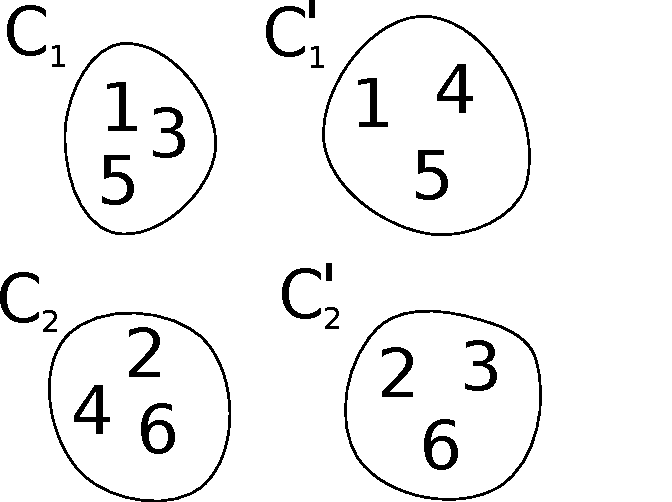
\includegraphics[scale=0.47]{./figs/ex_1.pdf} & 
			\hspace{-14mm}
			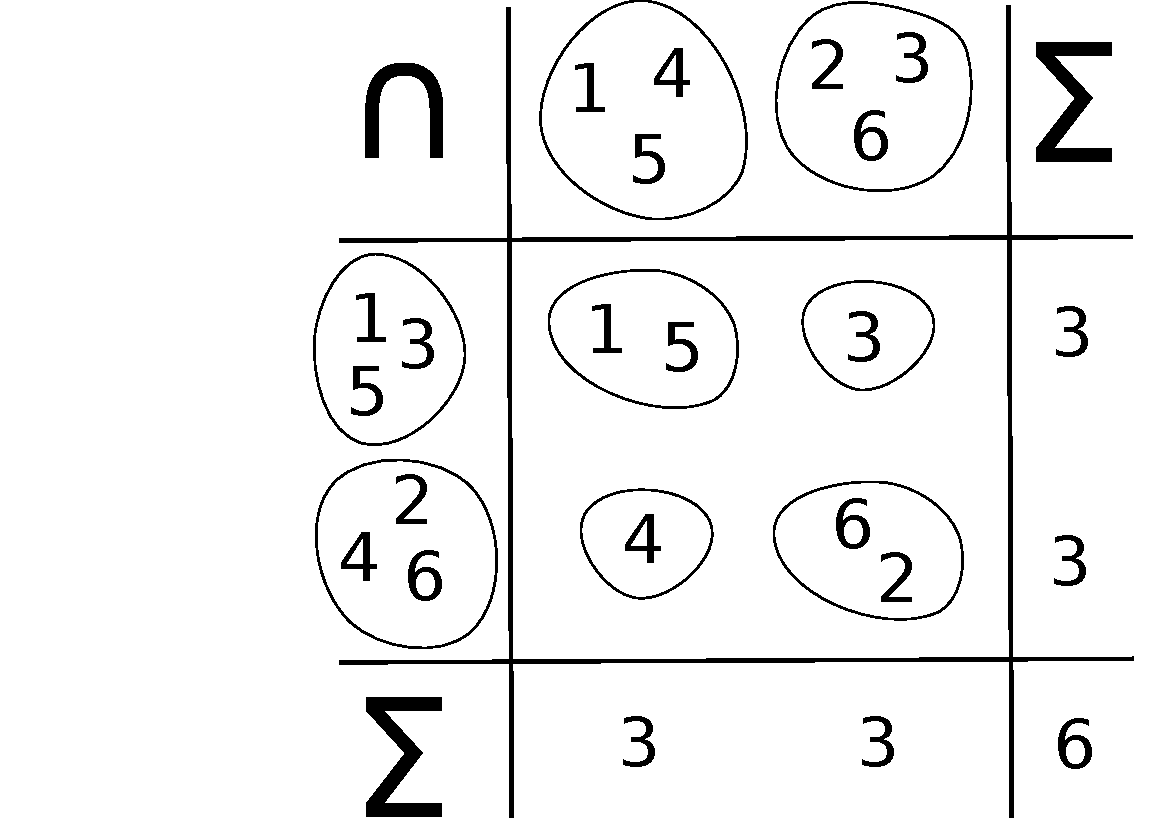
\includegraphics[scale=0.32]{./figs/contingence_3.pdf} \\
		\end{tabular}
	\end{block}
\end{frame}


\subsection{Nuevo índice de validación externa para clusters solapados}

\begin{frame}[t]
	\begin{block}{Factores del nuevo índice: OC}
	\begin{center}
		\visible<1-> Si ${p}$ representa la probabilidad de que 2 patrones se agrupen juntos, ¿qué esperamos si los patrones se agrupan en más de un cluster?
		
		\vspace{5mm}
		\begin{tabular}{l r}
			\multirow{2}{*}{
			\hspace{-5mm}
			\only<2> {${{p} = \frac{\sum\limits_{i=1}^{k} \binom{|c_i|}{2}}{\textbf{?}}}$ }
			\only<3->{${p} = \frac{\sum\limits_{i=1}^{k} \binom{|c_i|}{2}}{k\binom{N}{2}}$ }			
			}
			& \hspace{5mm}
			\visible<2-> {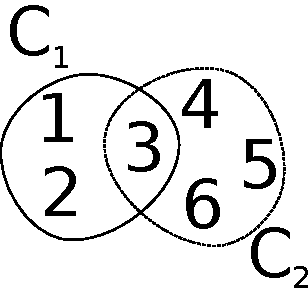
\includegraphics[scale=0.45]{./figs/ex_2_c__.pdf}} \\
			&
			\visible<3-> {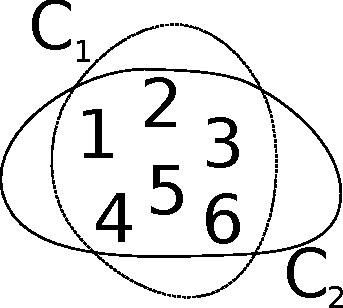
\includegraphics[scale=0.45]{./figs/ex_2_d__.pdf}} \\
		\end{tabular}
	\end{center}		
	\end{block}
\end{frame}

\begin{frame}[t]
    \begin{block}{{Propuesta de nuevo índice para clusters solapados}}
    \begin{itemize}    
 	\item[]<1-4>
 		\only<1> {${t} = \frac
		{\sum\limits_{i=1}^{k} 
			\sum\limits_{j=1}^{k^\prime} \binom{|c_i \cap c_j^{\prime}|}{2}}
		{\textbf{?}}$}
		\only<2> {${t} = \frac
		{\sum\limits_{i=1}^{k} 
			\sum\limits_{j=1}^{k^\prime} \binom{|c_i \cap c_j^{\prime}|}{2}}
		{\binom{N}{2} }$}

 		\only<3> {${t} = \frac
		{\sum\limits_{i=1}^{k} 
			\sum\limits_{j=1}^{k^\prime} \binom{|c_i \cap c_j^{\prime}|}{2}}
		{\binom{N}{2} min(k, k^\prime) }$}
		
 		\only<4> {${t} = \frac
		{\sum\limits_{i=1}^{k} 
			\sum\limits_{j=1}^{k^\prime} \binom{|c_i \cap c_j^{\prime}|}{2}}
		{\binom{N}{2} min(k, k^\prime) \frac{max(n,n^\prime)}{N}}$}



\item[]<5-> \visible<5->{
 		\only<5-> {${t} = \frac
		{\sum\limits_{i=1}^{k} 
			\sum\limits_{j=1}^{k^\prime} \binom{|c_i \cap c_j^{\prime}|}{2}}
		{\binom{N}{2} min(k, k^\prime) \frac{max(n,n^\prime)}{N}}$\\
		\vspace{3mm}		
		{${p} = \frac{\sum\limits_{i=1}^{k} \binom{|c_i|}{2}}{k\binom{N}{2}}$ }\\
		{${p^\prime} = \frac{\sum\limits_{j=1}^{k^\prime} \binom{|c^\prime_j|}{2}}{k^\prime\binom{N}{2}}$ }}
}
	\vspace{5mm}


    \end{itemize}
	\end{block}
\visible<6->{	\begin{block}{}
	{
	\begin{itemize}
		\item[] $	
		OC = \frac{ {t} }
		 {max({p},{p^{\prime}})}
			$
	\end{itemize}
	} 
	\end{block}}
	
\end{frame}